\subsection{Socketforbindelse}
\textbf{SocketConnection}
SocketConnection klassen implementerer asynkron læsning fra en socketforbindelse, samt synkron sending af data. Når der er oprettet forbindelse til en server (\gls{CS} i dette system) vil SocketConnection begynde at læse asynkront. Når der modtages data kaldes en handler, som kalder invoke på et "Data modtage" event. Dette event bruges af \textit{CommandListener}, som er beskrevet nedenfor.\\
Da læsning foregår asynkront vil resten af programmet ikke blive blokeret, hvilket er den optimale løsning, da der altid skal lyttes på socket forbindelsen efter nye kommandoer.\\
Klassen har også funktionalitet til at sende data. Dette gøres synkront. Der er ingen events relateret til at sende data.\\
SocketConnection implementerer også en række andre events, som bliver invoket når der er oprettet forbindelse, når forbindelsen bliver afbrudt og når der forekommer fejl.\\\\
 

\textbf{CommandListener}
Denne klasses ansvar er at håndtere den data der bliver modtaget af \textit{SocketConnection}. Klassen subscriber på \textit{SocketConnection} klassens "Data modtaget" event. Når der modtages data tjekker \textit{CommandListener} om der er modtaget en hel kommando XML streng. Er dette tilfældet, så bliver den afkodede kommando sendt til en kommando handler. Denne finder ud af, hvilken type command\footnote{Commands er nærmere beskrevet i afsnit \ref{COMMANDS} side \pageref{COMMANDS}} der er modtaget. Efterfølgende bliver der således raised et nyt event, som en bruger kan subscribe på, og have sin egen handler, som håndterer den modtagne kommando.\\
Der findes events for de følgende begivenheder:

\begin{itemize}
	\item Command modtaget
	\item Nyt produkt lavet
	\item Nyt produktkatalog
	\item Ny produktkategori lavet
	\item Produkt er slettet
	\item Produktkategori er slettet
	\item Produktkategori er modificeret
	\item Produkt er modificeret.
\end{itemize}

Selve kommandoen bliver sendt med, således brugeren selv kan håndtere denne.\\
På denne måde opnås en lav kobling. \textit{CommandListener} har ikke viden om, hvem der er subscribed på dens events, den raiser dem bare.

\begin{figure}[H]
	\centering
	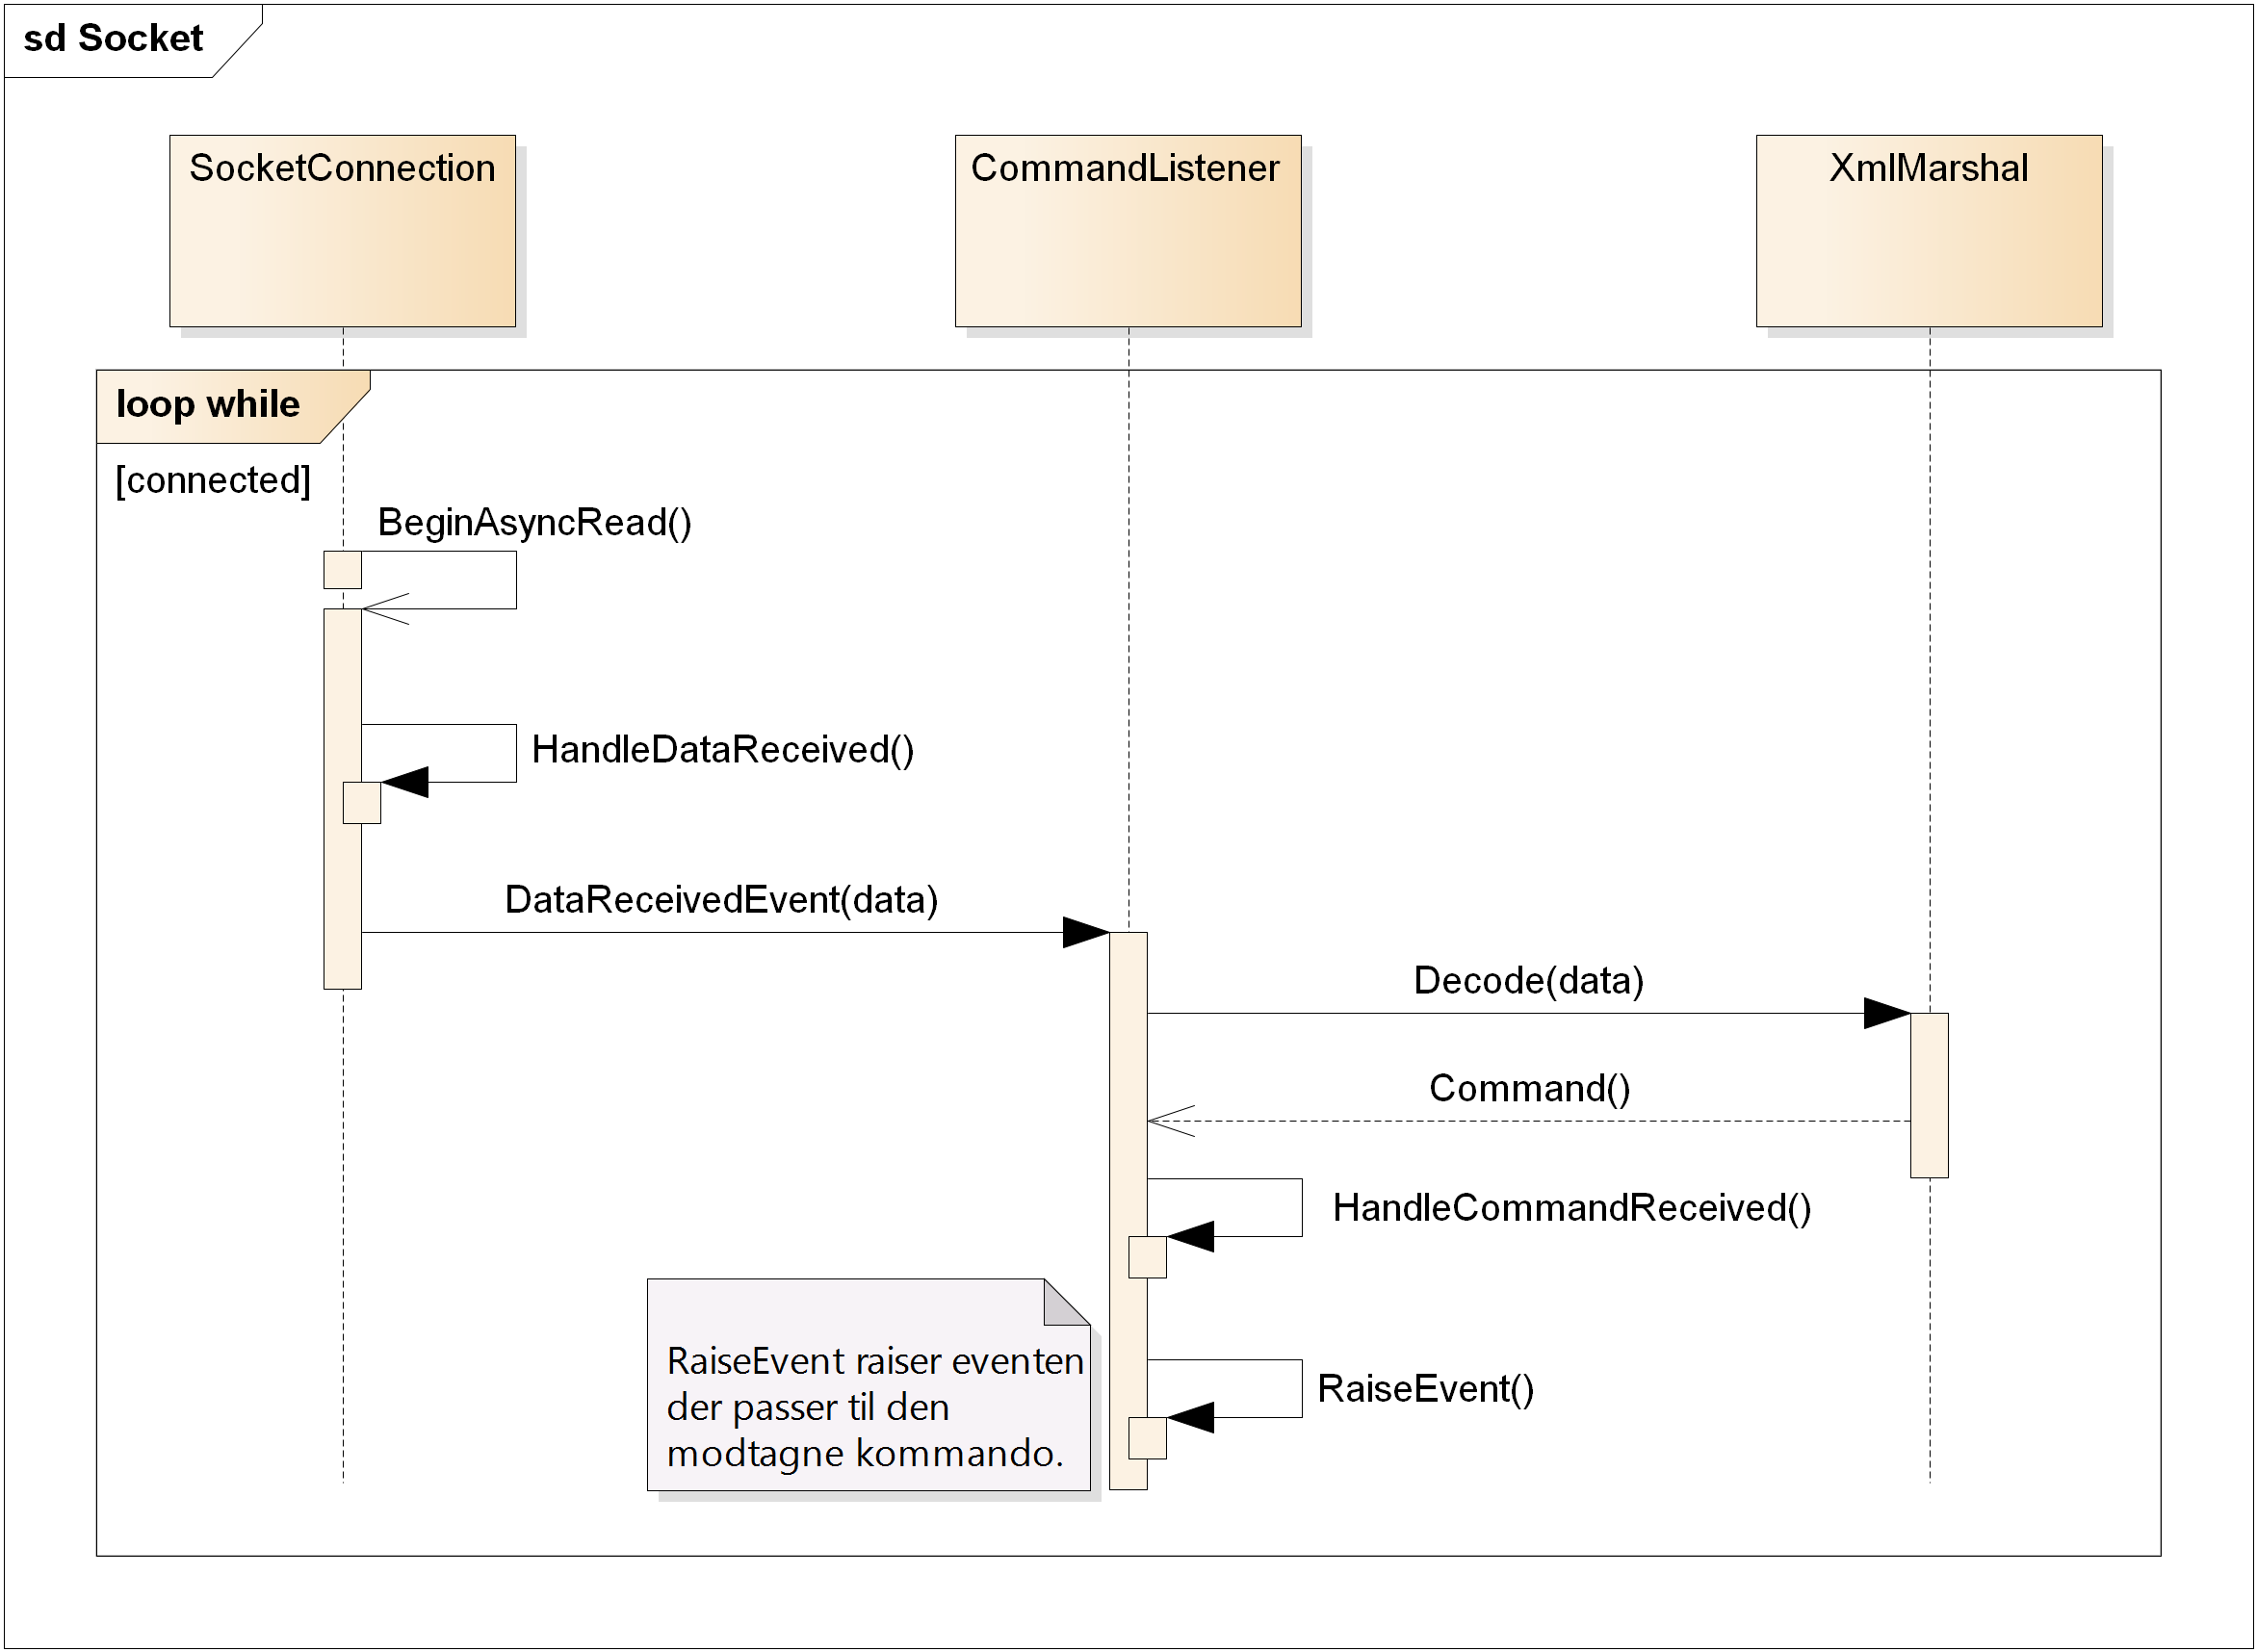
\includegraphics[width=1\textwidth]{Systemdesign/SharedLib/Images/Socket.png}
	\caption{Sekvensdiagram for socketforbindelsen}
	\label{fig:sockit}
\end{figure}

På diagrammet i figur \ref{fig:sockit} ses det hvordan data håndteres, når den modtages fra serveren. Ved SocketConnection vil read blive ved med at blive kaldt, medmindre der sker en fejl. I dette tilfælde vil et event om fejl blive raised. Se desuden hvordan dataen bearbejdes af modtageren i afsnit \ref{fig:DataReceive} side \pageref{fig:DataReceive}.
 